%!TEX root = foo-thesis.tex

\chapter{Prediction}
\label{chap:prediction}

Anhand der zuvor ermittelten Featurevektoren, bestehend aus Features mehrerer Scales und ggf. reduziert auf die Menge der \textit{uniquen} Punkte, soll nun jeweils die Klasse jedes Punktes vorhergesagt werden. Dazu kommt die zuvor geschriebene Featuresdatei zum Einsatz, aus der zunächst wieder die vollständigen Featurevektoren extrahiert werden müssen. Wie bei \cite{Zhiqiang.etal-2019} und \cite{Li.Cheng-2018} wird in diesem Ansatz für die \textit{Prediction} ein \textit{Random Forest} verwendet, der in dortigen Experimenten einen probabilistischen Ansatz sowie ein \textit{Support-Vector-Machine}-Modell übertroffen hat. Ein \textit{Random Forest} zeichnet sich grundsätzlich durch eine hohe Robustheit gegenüber kleinen Abweichungen oder Anomalien aus, die besonders bei feinen Features, wie sie hier vorkommen, wünschenswert ist. \\
Die Grundlage eines \textit{Random Forest} ist der \textit{Decision Tree}. Ein solcher einzelner Baum ist steuerbar über eine Menge von Parametern. Im Allgemeinen erhält er nur eine Teilmenge der Trainingsdaten und auch nur eine Teilmenge der Features zur Betrachtung. Anschließend wird er daraufhin trainiert, durch eine Reihe von Entscheidungen - im rein numerischen Fall basierend auf geeigneten Schwellwerten - die Klasse der Eingabe anhand der ihm zur Verfügung gestellten Features zu bestimmen. Um \textit{Overfitting}, also eine zu starke Spezialisierung auf die Trainingsdaten und damit zu geringe Generalisierung, zu vermindern, kann auch die maximale Anzahl an Entscheidungen - die Tiefe des Baums - festgelegt werden. \\
Für sich genommen ist ein einzelner Baum nur bei einigen Features zu einer sinnvollen Entscheidung für eine Klasse geeignet, bei anderen Features ist diese eher zufällig. Dies wird im \textit{Random Forest} dadurch ausgenutzt, dass jener oft aus Hunderten oder mehr unkorrelierten \textit{Decision Trees} besteht. Jeder von diesen trifft eine Entscheidung, die letztliche Entscheidung des gesamten Modells ergibt sich als Mehrheitsmeinung (\textit{Majority Vote}) dieser Einzelvorhersagen. Das Zusammenspiel aus \textit{Expertenmeinungen} jeweils spezialisierter Bäume und eher zufälligen Entscheidungen der restlichen Bäume ist einer der wesentlichen Gründe für die Stabilität des Modells \citep{Breiman-2001}.\\
Die einzigen beiden Parameter, die für diesen Ansatz manuell gesetzt wurden, sind die Gesamtzahl der \textit{Decision Trees}, aus denen der \textit{Random Forest} besteht, sowie die maximale Tiefe pro Baum. Die Anzahl der Bäume liegt für die Experimente bei 100. Es wurden auch höhere Zahlen getestet, die aber keine signifikanten Steigerungen bei der Qualität der \textit{Predictions} brachten. Während dieser Wert dem von \cite{Zhiqiang.etal-2019} gleicht, liegt die maximale Tiefe eines Baums hier bei 15 statt bei 10. Dies kann damit begründet werden, dass im vorliegenden Ansatz deutlich größere Featurevektoren genutzt werden: statt insgesamt 48 beinhalten sie hier 240 Werte (5 Scales á 48 \textit{Frequencies}). Eine noch größere Tiefe brachte bei Versuchen allerdings keine Verbesserungen mehr - im Gegenteil scheint dann ein \textit{Overfitting} auf die Trainingsdaten stattzufinden durch zu spezialisierte Entscheidungen pro Baum. \\
Um mit dem Ungleichgewicht der Klassen umzugehen, das in Tabelle \ref{table:class_frequencies} konkretisiert wird, findet für das Training ein \textit{Sampling} der gewöhnlichen Straßenpunkte statt. Das bedeutet, von allen Straßenpunkten wird ein zufälliger Anteil behalten, der dem \textit{Random Forest} übergeben wird. Der Anteil für die durchgeführten Experimente ist dabei so groß, dass jene Punkte, die nicht die Klasse Straße besitzen, etwa ein Zehntel der Gesamtpunkte ausmachen. Dies stellt eine Abwägung dar von der Reduktion des Ungleichgewichts gegenüber der Beibehaltung realistischer Klassenverhältnisse. \\\\
Für die \textit{Predictions} mittels \textit{Random Forest} wird das Paket \textit{scikit-learn} verwendet, das vielseitige Funktionalitäten im Bereich des maschinellen Lernens bietet. Die Python-Skripte des Ansatzes lassen sich über eine Kommandozeilen-Schnittstelle bedienen:
\begin{itemize}
    \item Es kann ein \textit{Random Forest} erstellt und trainiert werden. Dazu muss eine Featuresdatei eingelesen werden sowie eine Trainingspunktwolke mit den tatsächlichen Klassen. Darauf kann das Modell anschließend \textit{gefittet} werden, also seine Ausgaben an die gewünschten Ausgaben angenähert.
    \item Es kann ein \textit{Random Forest} getestet werden auf seine Qualität. Dazu muss neben dem trainierten Modell erneut eine Featuresdatei eingelesen werden sowie die zugehörige Testpunktwolke mit den tatsächlichen Klassen. Anschließend findet die \textit{Prediction} der Punktklassen durch den \textit{Random Forest} statt, was mit den erwarteten Klassen abgeglichen und in Form von Metriken pro Klasse evaluiert wird. Zu den hier verwendeten Metriken siehe Kapitel \ref{chap:eval}.
    \item Es kann auch ein anderes Modell auf seine Qualität getestet werden. Dazu wird neben der Testpunktwolke mit den tatsächlichen Klassen nur die \textit{Prediction}-Punktwolke benötigt mit den vorhergesagten Klassen. Damit werden anschließend ebenfalls Metriken für die einzelnen Klassen berechnet. Diese Option wurde vorrangig eingeführt, um mit den \textit{Predictions} von \texttt{PointNet} analog zu arbeiten wie mit denen des eigenen Ansatzes. Dies umfasst neben der Ermittlung derselben Metriken auch ein mögliches, identisch durchgeführtes \textit{Postprocessing}.
    \item Es können die Klassen einer noch nicht annotierten Punktwolke vorhergesagt werden. Dazu muss neben dem gewünschten Modell die entsprechende Featuresdatei eingelesen werden sowie die Punktwolke selbst zum Schreiben der Klassen. Dieser \textit{Prediction}-Teil ist für einen potenziellen regelmäßigen Einsatz auf der Plattform der bedeutsamste.
\end{itemize}
Beim Testen sowie der \textit{Prediction} des Modells besteht die Möglichkeit, über ein \textit{Flag} zu bestimmen, ob ein \textit{Postprocessing} der vorhergesagten Klassen stattfinden soll oder nicht. Genaue Erläuterungen zu dessen Funktionsweise finden sich in Kapitel \ref{chap:postproc}. In Abbildung \ref{fig:prediction} ist der grundsätzliche Ablauf einer solchen \textit{Prediction} dargestellt.

\begin{figure}[!ht]
    \centering
    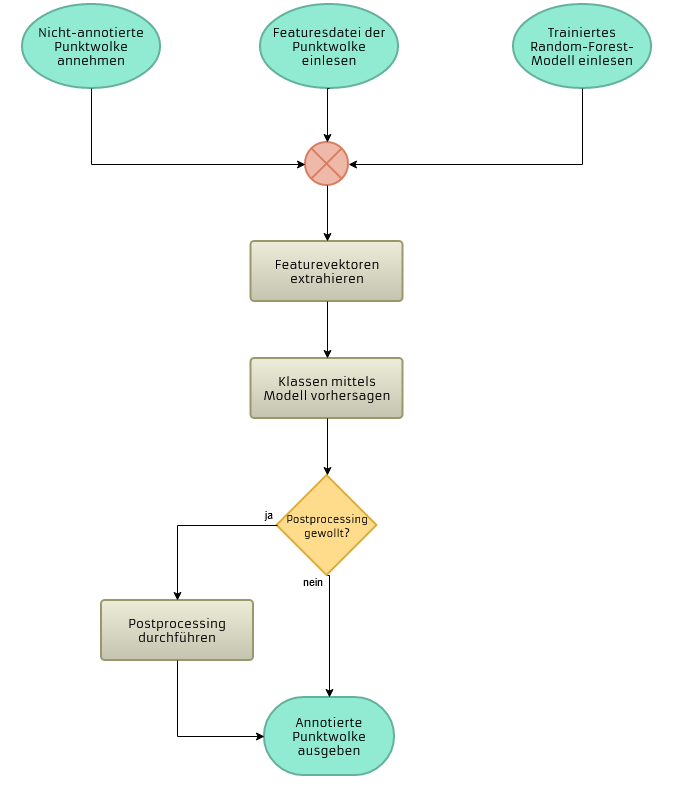
\includegraphics[width=0.95\textwidth]{graphics/flowchart_prediction}
    \caption{Eine Übersicht des Ablaufs einer Prediction.}
    \label{fig:prediction}
\end{figure}